%%%%%%%%%%%%%%%%%%%%%%%%%%%%%%%%%%%%%%%%%%%%%%%%%%%%%%%%%%%%%%%%%%%%%%%%%%%%%%%%
%2345678901234567890123456789012345678901234567890123456789012345678901234567890
%        1         2         3         4         5         6         7         8

%\documentclass[letterpaper, 10 pt, conference]{ieeeconf}  % Comment this line out if you need a4paper

\documentclass[a4paper, 10pt, conference]{ieeeconf}      % Use this line for a4 paper

\IEEEoverridecommandlockouts                              % This command is only needed if
                                                          % you want to use the \thanks command

\overrideIEEEmargins                                      % Needed to meet printer requirements.

%In case you encounter the following error:
%Error 1010 The PDF file may be corrupt (unable to open PDF file) OR
%Error 1000 An error occurred while parsing a contents stream. Unable to analyze the PDF file.
%This is a known problem with pdfLaTeX conversion filter. The file cannot be opened with acrobat reader
%Please use one of the alternatives below to circumvent this error by uncommenting one or the other
%\pdfobjcompresslevel=0
%\pdfminorversion=4

% See the \addtolength command later in the file to balance the column lengths
% on the last page of the document

% The following packages can be found on http:\\www.ctan.org
\usepackage{graphics} % for pdf, bitmapped graphics files
%\usepackage{epsfig} % for postscript graphics files
%\usepackage{mathptmx} % assumes new font selection scheme installed
%\usepackage{times} % assumes new font selection scheme installed
\usepackage{amsmath} % assumes amsmath package installed
\usepackage{amssymb}
\usepackage{graphicx}  % assumes amsmath package installed
\usepackage{enumitem}
\usepackage{tikz}
\usepackage{amsfonts}
\usepackage{multirow}
\usepackage{float}
\usetikzlibrary{arrows,automata}
\usepackage{pgfplots}
\usetikzlibrary{intersections}


%\usepackage[utf8]{inputenc}

\title{\LARGE \bf
Multi-Modal Simultaneous Forecasting\\%
of Vehicle Position Sequences using Social Attention
}


\author{Jean Mercat$^{1, 2}$, Nicole El Zoghby$^{1}$, Guillaume Sandou$^{2}$, Thomas Gilles$^{1, 3}$,\\%
Dominique Beauvois$^{2}$, and Guillermo Pita Gil$^{1}$% <-this % stops a space
%\thanks{*This work was made in collaboration with L2S and Renault SAS}% <-this % stops a space
\thanks{$^{1}$ Department of data fusion,
        Technocentre Renault, 78280 Guyancourt, France
        {\tt\Small \{Jean.Mercat, Thomas.Gilles, Nicole.El-Zoghby, Guillermo.Pita-Gil\}@renault.com}}%
\thanks{$^{2}$ Laboratoire des signaux et des syst\`emes,
        Centrale-Sup\'elec, 91192 Gif sur Yvette, France
        {\tt\Small \{Jean.Mercat, Guillaume.Sandou, Dominique.Beauvois\}@centralesupelec.fr}}%
\thanks{$^{3}$ \'Ecole polytechnique,
        Route de Saclay, 91128 Palaiseau
        {\tt\Small Thomas.Gilles@polytechnique.edu}}%
}

\begin{document}


\tikzset{
    state/.style={
           rectangle,
           draw=black, very thick,
           minimum height=2em,
           inner sep=2pt,
           text centered,
           },
    name plot/.style={every path/.style={name path global=#1}}
}

\pgfmathdeclarefunction{dnorm}{2}{%
  \pgfmathparse{1/(#2*sqrt(2*pi))*exp(-((x-#1)^2)/(2*#2^2))}%
}




\maketitle
\thispagestyle{empty}
\pagestyle{empty}


%%%%%%%%%%%%%%%%%%%%%%%%%%%%%%%%%%%%%%%%%%%%%%%%%%%%%%%%%%%%%%%%%%%%%%%%%%%%%%%%
\begin{abstract}

Vehicle trajectory forecasting models use a wide variety of frameworks for interaction and multi-modality.
They rely on various representations of the road scene and definitions of maneuvers.
In this paper we present a simple model that
simultaneously forecasts each vehicle position on a road scene as a sequence
of multi-modal probability density functions.
This relies solely on vehicle position tracks and does not define maneuvers.
We produce an easily extendable model that combines these predictive capabilities while surpassing state-of-the-art
results.
Its architecture uses multi-head attention to account for complete interactions between all vehicles,
and long short-term memory (LSTM) layers for encoding and forecasting.

\end{abstract}


%%%%%%%%%%%%%%%%%%%%%%%%%%%%%%%%%%%%%%%%%%%%%%%%%%%%%%%%%%%%%%%%%%%%%%%%%%%%%%%%
\section{INTRODUCTION}

Automation of driving tasks aims for safety and comfort improvements.
For that purpose, most Autonomous Driving (AD) system relies on the anticipation of the
traffic scene movements.
%Here we present a forecasting model that produce multimodal stochastic predictions for all vehicles of a partially
%observed road scene.
The AD system uses sensors for perception to produce an interpreted representation of its surroundings.
For this work the surroundings are composed of all tracks of observed vehicle positions for the past
few seconds.
Using this simple representation without constraint on the input data, the produced output is a multimodal stochastic
forecast for each vehicle future positions.

In most forecasting applications, only the ego vehicle trajectory is predicted.
However, avoiding collisions can only be made with forecasts for all participants.
In some applications, to predict the whole scene, each vehicle trajectory can be predicted separately with the same
model.
However, this means that only one-way interactions (others to predicted vehicle) are modeled.
Therefore, simultaneous forecast of all perceived vehicles takes better accounts of interactions.

In a scene observed from an ego vehicle, the quality of the perceived information about the
surroundings of each vehicle is uneven.
The model forecasting a vehicle trajectory at the boundary of the field of view should not assume
that there is nothing where nothing is seen.


Some of the information that determines the future trajectories of the observed vehicle cannot be observed.
Therefore, the predictions are inherently uncertain.
We classify the uncertainties in two kinds: small variations around a mode and modes.
The first kind are the continuous uncertainties that are present at each step of the process such as perception,
estimation, and some model approximations.
The second kind are discrete local maxima of probability density.
They stand for occurrences of choices, for example, a driver chooses a lane,
or the perception system chooses a classification.
The forecasts represent both source of uncertainties with
density probability functions in the form of Gaussian mixtures.


This works combines stochastic multimodal forecasting with simultaneous forecasts of the whole scene
without assuming anything in unobserved areas.
This produces a model that simulates two-way interactions in time between all participants
while accounting for uncertainties from modes, and small variations.
It relies on a very simple representation of the environment that is easily extendable.

\section{Related work}

\textbf{The evolution} of road scene trajectory forecasting methods have progressively switched from kinematic, physics based models to learned
statistical frameworks.
The Kalman filters~\cite{Kalman1960} with various physical model is still widely used for short-term motion
forecast (less than 1 second) in the automotive industry.
However, to forecast with longer time horizon (about 5 seconds), statistical models have been used.
The survey~\cite{Lefevre2014} compares many statistical models for trajectory and maneuver forecast
with the most widely used models at that time being Hidden Markov Models (HMM) and Support Vector Machines (SVM).
Since then, recurrent neural networks (RNN) mostly using the Long Short-Term Memory~\cite{Hochreiter1997} (LSTM)
architecture have become the standard technology for statistical trajectory forecasting.
Its model free versatility has allowed the models to account for interactions between vehicles.
It has been used as a maneuver classifier in~\cite{Khosroshahi2016} and as a trajectory predictor in~\cite{Altche2017}.
The current predictive LSTM-based networks commonly use an encoder/decoder architecture such as~\cite{Hu2018}
that builds a Conditional Variational Autoencoder for vehicle trajectory forecasting.

\textbf{Maneuver prediction} is a field of prediction in itself but is also used in trajectory forecasting
as a solution for multimodal forecasting~\cite{Hu2018, Houenou2013, Deo2018}.
The forecast for each mode is a trajectory conditioned to a maneuver.
The global forecast is made using a second module that estimate each maneuver probability to combine all
the trajectory forecasts.
This produces multi-modal forecasts indeed, however the predicted modes correspond to the predefined maneuvers.
%Therefore, only a careful choice of maneuver definitions could match them to
%the actual modes of the data distribution.
As shown in~\cite{Shouno2018}, the various modes in the trajectory data are very complex and numerous.
As a result, capturing them with a few predefined maneuvers is not likely to be enough.
Moreover, as stated in~\cite{Wissing2018} that addresses this issue, the time at which the maneuver occurs in the sequence
is not always defined.
This makes the predicted modes relative to the whole sequence and not to the position at each time step.

\textbf{Probability density function} express stochastic forecasts and control the
uncertainty without depending on sampling as in generative models~\cite{Kuefler2017} and models based on variational
auto-encoding~\cite{Lenz2017, Hu2018}.
As done in~\cite{Lenz2017, Deo2018}, our model expresses forecasts as Gaussian mixture density functions.
However, no maneuver definition as in~\cite{Deo2018} nor latent sampling is needed for our model to
produce a multimodal distribution.

\textbf{Attention mechanisms} in neural networks have been able to introduce inter-dependencies within a variable
number of inputs.
It has been used for pedestrian trajectory forecasting in~\cite{Vemula2018} with spatiotemporal graphs and
in~\cite{Sadeghian2018a} with spatial and social attention using a generative neural network.
In~\cite{Sadeghian2018b}, attention over top-view road scene images for car trajectory forecasting is used.
Multi-head attention mechanism has been developed in~\cite{Vaswani2017} for sentence translation.
In~\cite{Messaoud2019} a mechanism called non-local  multi-head attention is developed.
However, this is a spatial attention that does not allow vehicle to vehicle attention.


In the present architecture, we use a multi-head social attention mechanism working together with
recurrent neural networks to forecast in the form of sequences of multi-modal position probability density
functions.

\section{Objectives}
\label{sec_obj}

The goal is to build a road scene vehicles trajectory prediction model that is versatile yet accurate.
It relies on vehicle tracks that are produced by a perception, fusion and tracking system.
For versatility, the inputs and the architecture are kept simple.
Therefore, the model is easy to adapt to more complete inputs, so it can be improved for specific applications.
The forecasts are made simultaneously for all vehicles in the road scene and accounts for interactions.
Moreover, it is commonly admitted that future trajectories are stochastic with a multimodal distribution.
The forecasts also account for that without depending on any maneuver supervision nor random sampling.
The model is able to work with road scene observations that contain different numbers of vehicles without ordering.

%\subsection{Global definition of the prediction function}
\label{sec_inout}


\textbf{The inputs} are sequences of all vehicle $(x, y)$ positions in a road scene.
At each time $t_0$, we consider an observation history with a fixed observation frequency and a
fixed number of observations $n_{\text{hist}}$.
The history trajectory is written $\{(x, y)_{k}\}_{k=-n_{\text{hist}}+1, 0}$.
The coordinate system is centered on the ego vehicle position at $t_0$.

\textbf{The outputs} are sequences of $n_{\text{pred}}$ Gaussians mixtures for each vehicle.
It is expressed with a sextuplets $(\hat{x}, \hat{y}, \sigma_x, \sigma_y, \rho, p)$
for each vehicle, at each forecast step and for each mixture component.
It defines a Gaussian component $(\mathcal{N}((\hat{x}, \hat{y}), \Sigma), p)$ with
    \[\Sigma =
    \left( \begin{matrix}
        \sigma_x^2 & \rho \sigma_x \sigma_y \\
        \rho \sigma_x \sigma_y & \sigma_y^2
    \end{matrix}\right)
    \]
the covariance matrix, and $p$ the mixture weight such that for $M$ components, $\sum_{m=1}^M{p_m} = 1$.

\textbf{The forecasting model} is a set of functions $pred_\theta : inputs \rightarrow outputs$.
The inputs and outputs sets are defined with the cartesian products:
\begin{equation*}
    \begin{split}
    \text{inputs} &\in \left( \mathbb{R}^{2} \right)^{n_{\text{hist}} \times n_{\text{veh}}}\\
    \text{outputs} &\in \bigg(\Big( {
    \underbrace{\vphantom{\mathbb{R}_+^{2}}
        \mathbb{R}^{2}}_{\hat{x}, \hat{y}}} \times
    {\underbrace{
        \mathbb{R}_+^{2}}_{\sigma_x, \sigma_y}} \times
    {\underbrace{\vphantom{\mathbb{R}_+^{2}}
        [-1, 1]}_{\rho}}\Big)^{n_{\text{mix}}} \times
    {\underbrace{\vphantom{\mathbb{R}_+^{2}}
    \Delta^{n_{\text{mix}}}}_{p}} \bigg)^{n_{\text{pred}} \times n_{\text{veh}}}
    \end{split}
\end{equation*}

$\Delta^{n_{\text{mix}}}$ is the $n_{\text{mix}}$ elements simplex:
\[\Delta^{n} = \Big\{(p_1,\dots,p_n)\in\mathbb{R}^{n}~\Big|~\sum_{i = 1}^n p_i = 1,~ p_i \ge 1~ \forall i\Big\}\]

The $pred_\theta$ function set is defined as a neural network with weights $\theta$.
It is invariant to permutations along the vehicle axis and it
is defined for all number of vehicles $n_{\text{veh}}$ and forecast steps $n_{\text{pred}}$.


\section{Model architecture}

This model uses an encoder-decoder structure.
It is based on LSTM networks for encoding and forecasting.
Here, we propose to add two multi-head self-attention layers to this architecture for interaction awareness.
The first attention layer is added after encoding to incorporate current interactions in the encoded vector of each vehicle.
The second attention layer is added after forecasting and before decoding.
This allows the forecast position sequences to remain coherent with each other.

The benefit of using self-attention layers for interactions is that the whole model computations are defined for
any number of vehicles and invariant to their ordering in the input tensor.
Since all other computations are the same for each vehicle, this property is kept throughout the whole model.

\subsection{Global architecture}


\begin{figure}[ht]
   \centering
    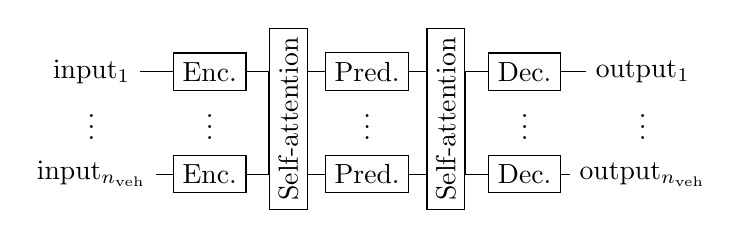
\begin{tikzpicture}
        \node(X1){input$_1$};
        \node[below of=X1, node distance=0.6cm](X2){$\vdots$};
        \node[below of=X2, node distance=0.7cm](X3){input$_{n_{\text{veh}}}$};

        \node[draw, right of=X1, node distance=1.5cm, rectangle](ENC1){Enc.};
        \node[below of=ENC1, node distance=0.6cm](ENC2){$\vdots$};
        \node[draw, right of=X3, node distance=1.5cm, rectangle](ENC3){Enc.};

        \path (X1) edge (ENC1);
        \path (X3) edge (ENC3);


        \node[draw, rectangle, right of=ENC2, node distance=1cm](TRANS1){\rotatebox{90}{Self-attention}};

        \draw (ENC1.east) -| (TRANS1.west);
        \draw (ENC3.east) -| (TRANS1.west);


        \node[draw, right of=ENC1, node distance=2cm, rectangle](PRED1){Pred.};
        \node[below of=PRED1, node distance=0.6cm](PRED2){$\vdots$};
        \node[draw, below of=PRED2, node distance=0.7cm, rectangle](PRED3){Pred.};

        \draw (TRANS1.east) |- (PRED1.west);
        \draw (TRANS1.east) |- (PRED3.west);

        \node[draw, rectangle, right of=PRED2, node distance=1cm](TRANS2){\rotatebox{90}{Self-attention}};

        \draw (PRED1.east) -| (TRANS2.west);
        \draw (PRED3.east) -| (TRANS2.west);

        \node[draw, right of=PRED1, node distance=2cm, rectangle](DEC1){Dec.};
        \node[below of=DEC1, node distance=0.6cm](DEC2){$\vdots$};
        \node[draw, below of=DEC2, node distance=0.7cm, rectangle](DEC3){Dec.};

        \draw (TRANS2.east) |- (DEC1.west);
        \draw (TRANS2.east) |- (DEC3.west);

        \node[right of=DEC1, node distance=1.5cm](Y1){output$_1$};
        \node[right of=DEC2, node distance=1.5cm](Y2){$\vdots$};
        \node[right of=DEC3, node distance=1.5cm](Y3){output$_{n_{\text{veh}}}$};

        \draw (DEC1.east) -- (Y1.west);
        \draw (DEC3.east) -- (Y3.west);

%        \draw[decorate,decoration={brace,mirror}] (X1.north west) -- node[left=10pt] {$X$} (X3.south west);
    \end{tikzpicture}
    \caption{Bloc representation of our forecasting model.
    Inputs are the sequence of past observations of each vehicle.
    Outputs are the matching forecasts.}
    \label{sch_whole_model}

\end{figure}

The figure~\ref{sch_whole_model} is a bloc representation of our forecasting model.
It is described in four parts: Encoder, Self-Attention, Predictor, and Decoder.
The two self-attention layers are different layers with the same architecture whereas the
encoder, predictor, and decoder are the same for every input.

\subsection{Encoder}

The encoder should act as a current state estimation for each vehicle using the past observation sequences.
This state is an intermediary vector of the neural network and is difficult to interpret.
However, since it should encode the current state with at least the information of position, kinematic state,
and interaction features, it should have a sufficient dimension, we chose 128.
The input $(x, y)$ position sequences are fed to a one dimensional convolutional layer with a kernel
of size 3 sliding over the time dimension that creates sequences of 128 features for each vehicle.
Then each feature sequence is encoded with a Long Short-Term Memory (LSTM)~\cite{Hochreiter1997}
into a vector of 128 features for each vehicle.


\subsection{Self-attention}
\label{sec_self_attention}


The multi-head self-attention layers allow vehicle interactions while keeping independence from their number
and ordering.
This mechanism is described in~\cite{Vaswani2017} where it is applied on sentence translation.
In this section we explain its use for vehicle interactions.
We tried $4$ and $8$ attention heads for both layers and used $4$ in the application.
The computations made by each attention head is represented on figure~\ref{sch_selfattention} and are detailed below.

\begin{figure}[ht]
    \centering
    \begin{tikzpicture}[scale=0.8, every node/.style={scale=0.8}]
        \node(X1){input$_1$};
        \node[below of=X1, node distance=2cm](X2){$\vdots$};
        \node[below of=X2, node distance=2cm](X3){input$_{n_{\text{veh}}}$};

        \coordinate[right of= X1, node distance=1cm](X1b){};

        \draw (X1) -- (X1b);

        \node[draw, right of=X1b, node distance=1cm](LQ1){$L_{q}$};
        \node[draw, above of=LQ1, node distance=1cm](LV1){$L_{v}$};
        \node[draw, below of=LQ1, node distance=1cm](LK1){$L_{k}$};

        \draw (X1b) -- (LV1);
        \draw (X1b) -- (LQ1);
        \draw (X1b) -- (LK1);

        \node[right of=LV1, node distance=1cm](V1){$\mathbf{v}_1$};
        \node[right of=LQ1, node distance=1cm](Q1){$\mathbf{q}_1$};
        \node[right of=LK1, node distance=1cm](K1){$\mathbf{k}_1$};

        \draw (LV1) -- (V1);
        \draw (LQ1) -- (Q1);
        \draw (LK1) -- (K1);


        \coordinate[right of= X3, node distance=1cm](X3b){};

        \draw (X3) -- (X3b);

        \node[draw, right of=X3b, node distance=1cm](LQ3){$L_{q}$};
        \node[draw, above of=LQ3, node distance=1cm](LV3){$L_{v}$};
        \node[draw, below of=LQ3, node distance=1cm](LK3){$L_{ k}$};

        \draw (X3b) -- (LV3);
        \draw (X3b) -- (LQ3);
        \draw (X3b) -- (LK3);

        \node[right of=LV3, node distance=1cm](V3){$\mathbf{v}_{n_{\text{veh}}}$};
        \node[right of=LQ3, node distance=1cm](Q3){$\mathbf{q}_{n_{\text{veh}}}$};
        \node[right of=LK3, node distance=1cm](K3){$\mathbf{k}_{n_{\text{veh}}}$};

        \draw (LV3) -- (V3);
        \draw (LQ3) -- (Q3);
        \draw (LK3) -- (K3);

        \coordinate[right of=V1, node distance=0.3cm](TOP){};
        \coordinate[right of=K3, node distance=0.3cm](BOT){};
        \draw[decorate,decoration={brace}] (TOP) -- node[left=5pt]{} (BOT);

        \node[right of=X2, text width=3cm, node distance=4.5cm](EQ){\footnotesize \[ V = \left( \begin{matrix}
                                                            \mathbf{v}_1 \\
                                                            \vdots \\
                                                            \mathbf{v}_{n_{\text{veh}}}
                                                          \end{matrix}\right) \]
                                                    \\
                                                   \footnotesize \[ Q = \left( \begin{matrix}
                                                            \mathbf{q}_1 \\
                                                            \vdots \\
                                                            \mathbf{q}_{n_{\text{veh}}}
                                                           \end{matrix} \right)\]
                                                    \\
                                                    \footnotesize \[K &= \left( \begin{matrix}
                                                            \mathbf{k}_1 \\
                                                            \vdots \\
                                                            \mathbf{k}_{n_{\text{veh}}}
                                                          \end{matrix} \right)\]
                                                  };

        \node[right of=EQ, node distance=1.5cm, rotate=90](EQ2){
        \footnotesize $\text{output}=\underset{\text{dim=last}}{\operatorname{Softmax}}\left(\frac{QK^T}{\sqrt{d_k}}\right)V$};

        \coordinate[right of =EQ2, node distance=1cm](CO2){};
        \coordinate[above of=CO2, node distance=2cm](CO1){};
        \coordinate[below of=CO2, node distance=2cm](CO3){};

        \node[right of=CO2, node distance=1cm](O2){$\vdots$};
        \node[right of=CO1, node distance=1cm](O1){output$_1$};
        \node[right of=CO3, node distance=1cm](O3){output$_{n_{\text{veh}}}$};

        \draw (CO1) -- (O1);
        \draw (CO3) -- (O3);

        \draw[decorate,decoration={brace, mirror}, xshift=-2cm] (CO1) -- node[left=15pt]{} (CO3);

    \end{tikzpicture}
    \caption{Schematic representation of one attention head computations.
    Blocs $L_{q}$, $L_{v}$, $L_{k}$ are matrix multiplications of the input vectors.}
    \label{sch_selfattention}
\end{figure}

Each vehicle should pay attention to specific features from a selection of the other vehicles.
This is made with four steps: pulling together specific features, identifying these feature collections,
enquiring among identifiers, and gathering the results.
Each head produces a different selection of features using a linear projection of
the input tensor resulting in the value tensor $V$.
To identify these features, a key tensor $K$ is associated to each value.
Then, each vehicle must select which other vehicle to pay attention to.
For that purpose a query $Q$ is produced to find a selection of keys.
The match score between a key and a query is the dot product is scaled with the square root of the key
dimension $\sqrt{d_k}$ and normalized with a softmax.
This produces an attention matrix that contains coefficients close to $1$ for matching queries and keys
and close to $0$ otherwise.
Finally, this matrix is used to gather the values from $V$.
Thus, the self-attention computation for each head is written:
\begin{equation}
    \text{output}=\underbrace{\underset{\text{dim}=\text{last}}{\operatorname{Softmax}}\left(\frac{QK^T}{\sqrt{d_k}}\right)}_{\text{attention matrix}}V
    \label{eq_selfattention}
\end{equation}
The outputs from all heads are concatenated and combined with a linear layer.
The resulting tensor is then added to the input as in residual networks.

\subsection{Predictor}
Tensors produced with the self-attention layer are repeated $n_{\text{pred}}$ times to be fed as time sequences
into a second LSTM layer.
This produces intermediary forecasts with some interaction awareness.
Within the forecast position sequences, vehicle interactions may have changed.
Thus, we placed a second multi-head self-attention layer before feeding the output to the decoder.

\subsection{Decoder}

Feature sequences are decoded with two convolutional layers with kernel size 1 and relu activations.
Finally, a last convolutional layer with kernel size 1 with a specific activation produces
the mixture of Gaussian output.
The output is described in section~\ref{sec_inout}.
Let $o_i$ be the $i^{\text{th}}$ coordinate of the output tensor before the activation function.
To constraint it, a specific activation function is applied on each coordinate at every time steps:
\begin{equation*}
    \begin{split}
        &\text{activation}(\{o_1, o_2, o_3, o_4, o_5, o_6\}_{i=1,n_{\text{mix}}})\\
        &~=\{(\hat{x}, \hat{y}, \sigma_x, \sigma_y, \rho, p)\}_{i=1,n_{\text{mix}}}\\
        &~=\Big\{(o_1, o_2, e^{\frac{o_3}{2}}, e^{\frac{o_4}{2}}, \operatorname{tanh}(o_5), \underset{i \in \text{mix}}{\operatorname{Softmax}}(o_6))_i\Big\}_{i=1,n_{\text{mix}}}
    \end{split}
\end{equation*}

\section{Loss and performance indicators}
\label{sec_loss}

The model is trained with the Adam optimizer~\cite{Kingma2015} that minimizes the negative log-likelihood (NLL) loss.
The usual performance indicators for such forecasting models are root mean squared error (RMSE),
mean absolute error (MAE), and negative log-likelihood (NLL).

\textbf{The RMSE} computation is made with equation~\eqref{eq_rmse} with $(x_k^i, y_k^i)$ the observed positions and
$(\hat{x}_k^i, \hat{y}_k^i)$ the most probable forecast positions of the $i^{th}$ sequence at time $t_k$.
$N$ is the number of sequences in the subset of the database on which the computation is made.

\begin{equation}
    \text{RMSE}(k) = \sqrt{\frac{1}{N}\sum_{i=1}^N{(x_k^i - \hat{x}_k^i)^2 + (y_k^i - \hat{y}_k^i)^2}}
    \label{eq_rmse}
\end{equation}

\textbf{The MAE} computation is made with equations~\eqref{eq_ade}.

\begin{equation}
    \begin{split}
        \text{MAE}_x(k) &=\frac{1}{N}\sum_{i=1}^N{|(x_k^i - \hat{x}_k^i)|}\\
        \text{MAE}_y(k) &=\frac{1}{N}\sum_{i=1}^N{|(y_k^i - \hat{y}_k^i)|}
    \end{split}
    \label{eq_ade}
\end{equation}

\textbf{The NLL} computation, at each forecast time $t_k$, for each Gaussian component centered on $(\hat{x}, \hat{y})$,  with the forecast
error\\
$\mathbf{d} = (d_x, d_y) = (x - \hat{x}, y -\hat{y})$ and the forecast error
covariance defined with $(\sigma_x, \sigma_y, \rho)$ is written:

\begin{equation}
    \begin{split}
        \text{NLL}(d_x, d_y, \Sigma) =
        & \frac{1}{2}\underbrace{\frac{1}{(1 - \rho^2)}\biggl(\frac{d_{x}^2}{\sigma_{x}^2} + \frac{d_{y}^2}{\sigma_{y}^2}
        -2 \rho \frac{d_{x} d_{y}}{\sigma_{x} \sigma_{y}}\biggr)
        }_{\mathbf{d_k}^T\Sigma_k^{-1}\mathbf{d_k}}\\
        & + \underbrace{\ln\biggl(\sigma_x\sigma_y\sqrt{1-\rho^2}\biggr)}_{\ln(\sqrt{|\Sigma_k|})}\\
        & + \ln(2\pi)
    \end{split}
    \label{eq_gauss_nll}
\end{equation}

The time index $k$ is dropped to improve readability.
The computation of the overall NLL value for all mixture components is written:

\begin{equation}
    \text{NLL}(d_x, d_y, \Sigma, p) = -ln\left( \sum_{m=1}^{n_{\text{mix}}} p_m e^{-\text{NLL}(d_{x_m}, d_{y_m}, \Sigma_m)} \right)
    \label{eq_multi_nll}
\end{equation}

The mean NLL (MNLL) over the test set is written:
\begin{equation}
    \text{MNLL} = \frac{1}{N}\sum_{i=1}^N{\text{NLL}_i}
\end{equation}

Minimizing the NLL loss maximizes the likelihood of the data for the forecast.
However, the optimization is not convex and one spurious local minimum that is often obtained is
%a unimodal distribution.
%Another spurious local minimum is
the overfitting of common behaviors on short horizons.

\emph{To avoid short-term overfitting}, the forecast variances are clipped with a 10cm minimum value.
This is an acceptable minimum variance, for long term forecasts that is not restrictive.
The gradient descent optimization with NLL loss tend to favor forecasts with small covariances and errors because the
NLL derivative is larger in those cases.
In~\cite{Lenz2017}, NLL overfitting has been obtained and has degraded the results, making the NLL value unreliable as a
performance indicator.
Clipping the variance values avoids large values of gradient for forecasts that where already well fitted.
This helps the optimization process avoiding this source of overfitting and allows us to rely on the NLL values.


%\emph{To encourage multimodal predictions}, an additional loss that penalize the similarity is added.
%A method using Detrimental Point Process (DPP) adapted from~\cite{Yuan2019} is used.
%The mode distance matrix $D \in \mathbb{R}^{n_{\text{mix}}, n_{\text{mix}}}$ defined as the
%difference between predicted modes positions:
%\begin{equation}
%    D_{i,j} = ||(x_i, y_i) - (x_j, y_j)||_2^2
%\end{equation}
%With $p$ the mixture factor vector
%%with values clipped within $[\epsilon, 1]$
%, and $I$ the identity matrix, the
%DPP kernel \\
%$L(D,p) = \exp(-\alpha~ diag(p) ~D~ diag(p))$ is used to define the similarity penalization:
%\begin{equation}
%    L_{diverse} = -tr(I - (L(D,p) + I)^{-1})
%\end{equation}
%
%In~\cite{Yuan2019}, using the mixing coefficient as a DPP kernel quality factor is said to favor major modes.
%This is detrimental if all modes are to be predicted.
%However, our goal is to predict the most likely future positions and not all possible future modes.
%
%\emph{To encourage multimodal predictions}, an additional loss that penalize the similarity is added.
%\begin{figure}[H]
%    \centering
%    \begin{tikzpicture}
%     \begin{axis}[
%            x=0.8cm,
%            y=5cm,
%            xmin=1,
%            xmax=10,
%            ymin=0,
%            ymax=0.4,
%            axis lines=center,
%            ticks=none,
%    %        xlabel={$k_t$},
%    %        ylabel={$f(k_t)$},
%    %        xlabel style={below right},
%    %        ylabel style={above left},
%            % (moved common `addplot' options here)
%            smooth,
%            domain=0:10,
%            samples=101,
%            no markers,
%        ]
%
%    % Draw curves
%    \addplot [thin, smooth, name path global=first] {dnorm(4,1)};
%    \addplot [thin, smooth, name path global=second] {dnorm(5.7,1.5)};
%
%    % Draw vertical line:
%    \path [name path global=first_line] ({rel axis cs:0,0}-|{axis cs:4,0}) -- ({rel axis cs:0,1}-|{axis cs:4,0});
%    \path [name path global=second_line] ({rel axis cs:0,0}-|{axis cs:5.7,0}) -- ({rel axis cs:0,1}-|{axis cs:5.7,0});
%
%    \path [name intersections={of=first_line and first}] (intersection-1) circle
%                coordinate (m1);
%    \path [name intersections={of=second_line and second}] (intersection-1) circle
%                coordinate (m2);
%
%    \node at ([shift={(6, 4)}]m1) [below right = 1cm of m1] {$\mathcal{N}_1$};
%    \node at ([shift={(6, 5)}]m2) [right = 1cm of m2] {$\mathcal{N}_2$};
%%    \draw [thick](m1) node [dot] {}
%%                -- (m1) node[dot, label:] {};
%%    \draw (m2) node[dot, label:right:$\mathcal{N}_2$] {};
%
%    \path [name intersections={of=first_line and second}] (intersection-1) circle
%                coordinate (p1);
%    \path [name intersections={of=second_line and first}] (intersection-1) circle
%                coordinate (p2);
%
%    \draw [dashed] (0, 0 -|  m1) node [dot]{}
%        -- (m1)                node [dot] {};
%    \draw [dashed] (0, 0 -|  m2) node [dot]{}
%        -- (m2)                node [dot] {};
%    \draw [very thick, <->] (0, 0 -|  p1) node [dot]{}
%        -- (p1)                node [dot, label=left:$p_{1/2}$] {};
%    \draw [very thick, <->] (0, 0 -|  p2) node [dot]{}
%        -- (p2)                node [dot, label=left:$p_{2/1}$] {};
%    %\draw [thick] (p2 -| 0, 0) node [dot, label=p1]{};
%    %\draw [thick, name intersections={of={second_line and first}}] ({rel axis cs:0,0}-|intersection-1) -- ({rel axis cs:0,1}-|intersection-1);
%    \end{axis}
%    \end{tikzpicture}
%
%    \caption{Graph of two Gaussian probability density functions (PDF). $p_{1/2}$ and $p_{2/1}$ are the values of one PDF computed
%    at the mean value of the other.}
%    \label{plt_gauss}
%\end{figure}
%
%Figure~\ref{plt_gauss} is an example representation of the intermediate computations used for
%the similarity penalization.
%For each couple of Gaussian mixture component $i$, and $j$ with $i \neq j$, the probability density function of one component
%is computed at the mean value of the other.
%This produces the two values $p_{i/j}$ and $p_{j/i}$.
%If the variance of one of the component $i$ is lower or equal to the clipping value defined in the previous paragraph,
%$p_{i/j}$ is set to $0$.
%The similarity penalization is defined as the mean value of the pair values product as written in equation~\eqref{eq_sim_loss}.
%\begin{equation}
%    \text{SIM} = \frac{1}{n_{\text{mix}}^2}\sum_{i \neq j} p_{i/j}p_{j/i}
%    \label{eq_sim_loss}
%\end{equation}
%
%For the closest horizon predictions, the variance is equal to the clipping value keeping the
%similarity penalization to $0$.
%This is a good behavior since the prediction at 0.2s does not need to be multimodal.
%As the prediction horizon increase, the variance also increase.
%Then the similarity penalization lowers the variances and pushes the mean values further from each other.
%This pushes predicted mixture of Gaussian toward a multimodal distribution.
%This penalization is on average several order of magnitude lower than the average loss and thus affects only slightly
%the predictions when they are multimodal.


%\subsection{Local attention}
%
%The attention mechanism makes combinations of each vehicles with every other.
%This is too broad and it should focus more on the local vehicles.
%To force this behavior, the equation~\eqref{eq_selfattention} is modified as follow:
%\begin{equation}
%    output=\underset{dim=last}{Softmax}\left(\frac{QK^T}{\sqrt{d_k}} - D\right)V
%    \label{eq_localattention}
%\end{equation}
%The distance tensor $D$ is a tensor whose last two axis form symetric matrices of coefficients
%$d_{i, j} = ||pos_{i} - pos_{j}||_2^2$ with $pos_i$ the position of the $i^{th}$ vehicle.
%It is substracted to the key/query product to lower the value corresponding distant vehicles.
%For the first attention layer, distances are computed directly from the last input positions.
%For the second attention layer, the output layer is used to extract positions from the predicted encoded sequences.
%The distance matrices are computed at every prediction step using these positions.
%Then local attention is computed with the same predicted encoded sequences and the associated distance matrices.
\section{Architecture discussion}

\subsection{Multi-head self-attention}

The general idea of this architecture is to use the good properties of the key-query self-attention layer to account for
interactions.
This offers flexibility to the model allowing powerful LSTM models to compute the features and predictions with
the fixed size inputs it demands while accepting a varying number of interacting vehicles without ordering.
All input vehicles are treated exactly the same way even if the perception of the road scene is only partial.
This allows the simultaneous forecast of each vehicle in the scene with a different and interdependent
social context for each.


This method is sometimes stated as computationally expensive because attention over $n$ objects relies on computations
involving an $n \times n$ attention matrix.
However, in our use cases, the number of objects is lower than $n=30$ and most of the times remains around $10$.
This small number makes global attention affordable in all of our test cases.
If another application uses a larger number of objects, local attention could be considered.
As stated in~\cite{Vaswani2017}, and shown in our application section~\ref{sec_application_attention}, multi-head
attention produces interpretable interactions with each head specializing on different interaction patterns.

\subsection{Hyperparameters}

This model is defined with a few specific hyperparameters that should be tuned: number of encoded features, number of
embedding and decoding layers and their activation functions, the number of heads in each self attention layer,
the number of mixture component in the output distribution and the error covariance clipping value.
Other choices have been made and should be questioned such as the data normalization (none is used),
the use of shortcut connections without layer normalization, the use of LSTM layers and some implicit choices
may have been overlooked.
Optimizing the hyperparameters with a thorough process could bring some improvements and
help understand the model but is not a part of the present study.
In this work, only the general concept was prioritized and the hyperparameters were chosen from experience.


\subsection{Maneuver free multimodal forecast}

With the present model, after defining a constant number of mixture components, they are differentiated solely with
the minimization of the loss.
%The loss is the sum of NLL and similarity penalisation.
The loss is only the NLL value averaged over time.
Thus, minimizing it pushes the predicted modes toward those of the data distribution.
What is forecast is not a mixture of trajectory density functions but a sequence of multimodal position
density functions.
There is a dependency between forecasts at time $t_k$ and at time $t_{k+1}$ but no explicit link between the modes
at those times.
Trajectories can be defined as the optimal transport path between the Gaussian mixture at time $t_k$ and the one at
time $t_{k+1}$.
To simplify, we make the assumption that mixture components centers define local maxima of the probability distributions
and can be tracked in time by matching similar mixture coefficients.

\subsection{How to extend this?}


The simplest extension is to add additional observations on each vehicle such as velocity, orientation, size, blinkers
and any other useful observation.
Since this is a model-free architecture, it can be done without changing it.


Another simple extension is to use a dictionary of encoders and decoders matching an input dictionary of moving
road scene object classes to be forecast.
No change is needed in the attention layer to allow attention between the different class of objects.


In the present architecture, self-attention produces keys, queries, and values from the same input to transform the
input value.
However, the keys and values can be extended with additional inputs with minimal change to the model.
The new input should be encoded with a separate encoder.
It may be for example, the encoding of the lane center line discretized as a sequence of
position points.
A bidirectional LSTM could be a good encoder architecture for this kind of input.
Then, each head of the first attention layer is extended with two additional linear layers $L_{vext}$ and $L_{kext}$,
both producing the same number of outputs and each with the same feature dimension
as the other linear layers from the attention head.
With this new input, extended keys and values are produced :
\begin{equation}
    \begin{split}
        \text{encoded}_{\text{ext}} &= \operatorname{extEncoder}(\text{input}_{\text{ext}})\\
        V_{\text{ext}} &= L_{v_{\text{ext}}}(\text{encoded}_{\text{ext}})\\
        K_{\text{ext}} &= L_{k_{\text{ext}}}(\text{encoded}_{\text{ext}})
    \end{split}
\end{equation}
These new keys and values can simply be concatenated to the head usual keys and values:
\begin{equation}
    \text{output}=\underset{\text{dim}=\text{last}}{\operatorname{Softmax}}\left(\frac{Q[K, K_{\text{ext}}]^T}{\sqrt{d_k}}\right)[V, V_{\text{ext}}]
    \label{eq_selfattention_extended}
\end{equation}
The output matches the vehicle features with an additional attention over the new input.


The ease of extension is one of the best asset of this model.
However, for conciseness and simplicity, only the core model is studied in the application.

\section{Application}

This model was implemented with the Pytorch library.
The NGSIM datasets US-101 and I-80 and its pre-processing were taken from
the published code accompanying the article~\cite{Deo2018}.
This also defines the dataset splitting into training, validation, and test sets.
Thus, a fair comparison with these results is made.
The dataset contains the tracks of all vehicle position on a road segment observed from a camera.
The pre-processing produces data that simulates observations from a given vehicle.
Each vehicle is alternatively chosen as the observing vehicle.
Its surroundings in adjacent lanes and within a given distance are recorded to produce a local road scene.
This road scene is tracked to produce 8 seconds sequences with all positions being recorded at a 5Hz frequency.
The 3 first seconds are used as past observations and the 5 next seconds are used as forecast supervision.



\begin{figure*}
        \centering
%        left btm right top
        \includegraphics[width=0.11\textwidth, clip, trim=0.49cm 5.06cm 43.5cm 0.1cm]{dessins/attention_look_front_131.pdf}
        \includegraphics[width=0.88\textwidth, clip, trim=10cm 4cm 0.1cm 1.55cm]{dessins/attention_look_front_131.pdf}
        \vspace{-10pt}
        \caption{
        A driving scene top view representation with all observed vehicles and the
        attention matrix for one head of the first attention layer.
        The attention that vehicle $i$ is giving to $j$ is drawn as an arrow from $i$ to $j$ with a width proportional
        to the attention coefficient and a color varying with its angle.
        A yellow circle represents the attention of one vehicle on itself (when $i=j$) with a radius proportional to
        the coefficient.
        The attention coefficients are represented as colors in the matrix on the left going from purple at $0$ to
        yellow at $1$.
        Past positions are represented in gray.
        Superposed forecast probability density functions are represented in blue shades in log scale.}
        \label{fig_veh_att}
        \vspace{-10pt}
\end{figure*}


\subsection{Global performance indicators}

\begin{table}
    \centering
    \caption{Comparison of RMSE, NLL and MAE results with baselines using the same dataset.
     *CSP(M) results were recomputed with some minor modifications for a fair comparison.}
    \begin{tabular}{l|l|ccccc}
        \hline
        \multicolumn{2}{l|}{\hspace{-5pt}Time horizon}                & 1s   & 2s   & 3s   & 4s   & 5s   \\
        \hline\hspace{-3pt}
        \multirow{3}{*}{\hspace{-5pt}RMSE\hspace{-3pt}} &\hspace{-3pt}CV~\cite{Mercat2019}      & 0.76 & 1.82 & 3.17 & 4.80 & 6.70 \\
                              &\hspace{-3pt}CSP(M)~\cite{Deo2018}*    & 0.57 & 1.25 & 2.10 & 3.17 & 4.49 \\
                              &\hspace{-3pt}GRIP~\cite{Li2019}        & \textbf{0.37} & \textbf{0.86} & \textbf{1.45} & \textbf{2.21} & \textbf{3.16} \\
                              &\hspace{-3pt}\textit{SAMMP$_4$}          & 0.49 & 1.10 & 1.84 & 2.77 & 3.93\\
                              &\hspace{-3pt}\textit{SAMMP$_8$}          & 0.49 & 1.10 & 1.84 & 2.77 & 3.93\\
%                              &\hspace{-3pt}$SAMMP_{MSE}$             & NA & NA & NA & NA & NA\\
        \hline
        \multirow{3}{*}{\hspace{-5pt}MNLL\hspace{-3pt}} &\hspace{-3pt}CV~\cite{Mercat2019}      & 0.82 & 2.32 & 3.23 & 3.91 & 4.46\\
                              &\hspace{-3pt}CSP(M)~\cite{Deo2018}*    & 1.78 & 3.35 & 4.24 & 4.88 & 5.47\\
                              &\hspace{-3pt}\textit{SAMMP$_4$}          & \textbf{0.45} & \textbf{1.11} & \textbf{1.73} & \textbf{2.26} & \textbf{2.72}\\
                              &\hspace{-3pt}\textit{SAMMP$_8$}          & \textbf{0.45} & \textbf{1.11} & \textbf{1.73} & \textbf{2.26} & \textbf{2.72}\\
%                              &\hspace{-3pt}$SAMMP_{MSE}$             & NA & NA & NA & NA & NA\\
        \hline
        \multirow{2}{*}{\hspace{-5pt}MAEx\hspace{-3pt}}&\hspace{-3pt}CV~\cite{Mercat2019}      & 0.42 & 1.17 & 2.19 & 3.44 & 4.90\\
                              &\hspace{-3pt}\textit{SAMMP$_4$}           & 0.29 & 0.74 & 1.28 & 1.96 & 2.82\\
                              &\hspace{-3pt}\textit{SAMMP$_8$}           & 0.29 & 0.74 & 1.28 & 1.96 & 2.82\\
%                              &\hspace{-3pt}$SAMMP_{MSE}$             & NA & NA & NA & NA & NA\\
        \hline
        \multirow{2}{*}{\hspace{-5pt}MAEy\hspace{-3pt}}&\hspace{-3pt}CV~\cite{Mercat2019}      & 0.11 & 0.21 & 0.31 & 0.39 & 0.48\\
                              &\hspace{-3pt}\textit{SAMMP$_4$}           & 0.06 & 0.11 & 0.15 & 0.19 & 0.22 \\
                              &\hspace{-3pt}\textit{SAMMP$_8$}           & 0.06 & 0.11 & 0.15 & 0.19 & 0.22 \\
%                              &\hspace{-3pt}$SAMMP_{MSE}$             & NA & NA & NA & NA & NA \\
        \hline
    \end{tabular}
    \label{tab_perf}
    \vspace{-10pt}
\end{table}

Table~\ref{tab_perf} reports results using the performance indicators defined in section~\ref{sec_loss}.
%These results are compared with the following baselines from the literature.
All compared models except for GRIP~\cite{Li2019} were trained and computed on the same dataset and evaluated with the same functions.
Since the model from~\cite{Deo2018} only forecasts the observing vehicle trajectory, only the errors for this vehicle are
being compared.

\textbf{Baselines}:

\emph{Constant velocity} (CV): We used a constant velocity Kalman filter with optimized parameters for forecasting
on the same data as described in~\cite{Mercat2019}.

\emph{Convolutional Social Pooling} (CSP(M)): We retrained the model from~\cite{Deo2018}.
It uses a maneuver classifier trained with preprocessed data that conditions a predictor for multimodal forecasts.
A forecast of the center vehicle trajectory is made with information from its social environment using the convolutional social
pooling mechanism.

\emph{Graph-based Interaction-aware Trajectory Prediction} (GRIP): We took the published results from~\cite{Li2019}.
It uses a spatial and temporal graph representation of the scene to make a maximum likelihood trajectory
prediction simultaneously fol all vehicles in the scene.
They obtain the best results in term of RMSE but it does not account for error estimation nor multimodality.

\emph{Social Attention Multi-Modal Prediction} (SAMMP): The model described in this article. SAMMP$_4$ and SAMMP$_4$
are the same model with 4 and 8 mixture components.


Our model forecasts multimodal probability density functions, thus the RMSE and MAE values that only relate to the most
probable forecast give only partial evaluations.
The mean NLL value however is relative to the whole distribution and is the preferred performance indicator.
As discussed in~\cite{Mercat2019}, this value is computed with different definitions in some other publications.
This is why results from~\cite{Deo2018} had to be recomputed.
MAE values are given for further comparisons.
They are less sensitive to very large errors that may be produced by observation errors that exist in the NGSIM dataset.
%Comparing them with RMSE values gives an idea of the error distribution.

\subsection{Attention interpretation}
\label{sec_application_attention}

The attention matrices give insights about the importance of some interactions.
Some of the heads roles can be rationalized by looking at the attention matrix it produces in different contexts.
For example, after every tested trainings of the model, one of the heads had specialized for front vehicle attention.
Figure~\ref{fig_veh_att} shows the attention scores as arrows between vehicles.
The main attention link always goes from one vehicle to the vehicle in front of it, or to itself if there is no
front vehicle.
The attention coefficient decreases with the increasing front vehicle distance.


\subsection{Multi-modal forecasting}

\begin{figure}[ht]
        \centering
%         trim=left botm right top
        \includegraphics[width=\linewidth, clip, trim=13.5cm 2.7cm 3.6cm 0.5cm]{dessins/multimodal_131.pdf}
        \vspace{-10pt}
        \caption{
        Another driving scene top view representation.
        Superposed forecast probability density functions of the ego position
        are represented in blue shades in log scale.
        Ground truth future positions are represented with a green line.
        }
        \label{fig_multimod}
        \vspace{-10pt}
\end{figure}


On the figure~\ref{fig_multimod}, the vehicle 0 aggressively overtakes the vehicle 3.
In this situation, the forecasts are multimodal.
The overtake could be aborted or be made less aggressively, also the last observations of
acceleration and turning could be the results of perception errors.


The NLL loss training is sufficient to produce this multimodal output and for simplicity this is what we used.
However, producing a better mode diversity could avoid mode averaging and mode collapsing.
This can be achieved with the introduction of a loss penalizing the mixture component similarity.
A good example of such a method is presented in~\cite{Yuan2019}.

%The predicted modes are relative to each position and not to the whole trajectory.
%However, it would be inconsistent for a series of modes describing a lane change to significantly change
%its probability over time.
%Thus, it is possible to draw predictions as trajectories by simply matching the modes with similar probabilities.
%This is the representation that is made on figure~\ref{fig_multimod}.
%In this case, the ego vehicle in blue is overtaking the


\section{CONCLUSIONS}

We proposed a road scene forecasting solution that produces multimodal probability function forecast
simultaneously for each vehicle of the scene.
Our method generates interpretable interaction models that could be extended to other road scene observations.
Experiments have surpassed state-of-the-art results with the NLL indicator.
This shows a good forecasting capacity as well as a good error estimation.
Future work will produce some of the proposed extensions and will experiment with the recently published datasets
such as Nuscenes~\cite{Nuscenes2019} and Argoverse~\cite{Chang2019}.


\subsubsection*{Acknowledgements} We are grateful to Edouard Leurent for his comments and corrections.

%The self-attention layers perform a convex combination of the input linear transformations.
%Interactive behaviors are not computed in this layer, it merely shares useful features among vehicles
%for the next layers to compute interactive behaviors.

%DumbPredictor_80_bis
%bias x [[-0.00379273  0.01119626]
% [-0.01110076  0.04440805]
% [-0.01560049  0.05443121]
% [-0.01796214  0.08589871]
% [-0.01867467  0.06826853]]
%bias y [[ 0.04342232 -0.00302752]
% [ 0.05297662  0.01595682]
% [ 0.06110188  0.01036763]
% [ 0.07085429  0.03495284]
% [ 0.07944416  0.0194513 ]]
%bias dist [[0.04421014 0.01260572]
% [0.05681306 0.05820303]
% [0.06842441 0.05716385]
% [0.0816729  0.10115807]
% [0.09105077 0.07447586]]
%bias \% [[9.05066888 2.58063485]
% [5.17432525 5.30091854]
% [3.72854133 3.11493774]
% [2.95013431 3.65396459]
% [2.31402351 1.89277796]]
%ADE [[0.05927011 0.29288597]
% [0.11125454 0.7365424 ]
% [0.15418566 1.28001025]
% [0.19065665 1.96462545]
% [0.22316268 2.82116637]]
%rmse most probable [0.48847378 1.09798007 1.83515226 2.76844685 3.93473846]
%rmse mean prob [0.50515508 1.10888453 1.83993835 2.76945954 3.93497273]
%nll [0.45118189 1.10969029 1.73349189 2.25706048 2.72143882]



%kalmantransformerGRU_8head_nll_46
%RMSE
%0.57939973 1.21238563 1.98451525 2.96286819 4.184847
%NLL
%-0.31314428  1.17847418  2.01719778  2.64240214  3.16598194





%CSLSTM no man:
%NLL:
%-2.0587, -0.3327, 0.7591,  1.4972,  2.0458,
%2.4783,  2.8292,  3.1230,  3.3774,  3.6037,
%3.8075,  3.9930,  4.1645,  4.3241,  4.4758,
%4.6186,  4.7540,  4.8831,  5.0065,  5.1244,
%5.2382,  5.3473,  5.4537,  5.5567,  5.6571
%RMSE:
%0.1052, 0.2111, 0.3223, 0.4436, 0.5680,
%0.6965, 0.8285, 0.9624, 1.1003, 1.2430,
%1.3916, 1.5469, 1.7099, 1.8814, 2.0619,
%2.2514, 2.4500, 2.6580, 2.8755, 3.1034,
%3.3415, 3.5895, 3.8484, 4.1189, 4.4014


%CSlstm_m_nll_3_ft:
%-2.2872, -0.5987,  0.4855,  1.2288,  1.7826,
%2.2160,  2.5693,  2.8672, 3.1257,  3.3550,
%3.5614,  3.7496,  3.9229,  4.0842,  4.2354,
%4.3779, 4.5128,  4.6409,  4.7631,  4.8820,
%4.9997,  5.1173,  5.2349,  5.3523, 5.4717
%
%0.1058, 0.2117, 0.3233, 0.4439, 0.5697,
%0.6978, 0.8292, 0.9651, 1.1060, 1.2528,
%1.4061, 1.5666, 1.7352, 1.9124, 2.0980,
%2.2925, 2.4963, 2.7099, 2.9335, 3.1675,
%3.4118, 3.6671, 3.9319, 4.2058, 4.4899


%NLL:
%-2.4959, -0.7516,  0.3690,  1.1446,  1.7165,
%2.1619,   2.5230,  2.8268,  3.0904,  3.3241,
%3.5533,  3.7383,  3.9091,  4.0685,  4.2180,
%4.3585, 4.4914,  4.6178,  4.7385,  4.8543,
%4.9658,  5.0735,  5.1777,  5.2793, 5.3783
%RMSE:
%0.1064, 0.2109, 0.3271, 0.4482, 0.5738,
%0.7052, 0.8404, 0.9794, 1.1226, 1.2712,
%1.4257, 1.5877, 1.7582, 1.9381, 2.1267,
%2.3232, 2.5289, 2.7452, 2.9715, 3.2069,
%3.4522, 3.7085, 3.9750, 4.2529, 4.5434

%DumbPredictor_local_att_28
%bias [0.01045633 0.05369709 0.09017866 0.10019906 0.06507623]
%bias (\% RMSE) [2.04381547 4.67443955 4.69984225 3.46073344 1.57623962]
%ADE [[0.06369706 0.30824296]
% [0.12183345 0.78371444]
% [0.1686192  1.36039922]
% [0.20843394 2.08387561]
% [0.24398934 3.00214884]]
%rmse [0.51160824 1.14873851 1.91875931 2.89531284 4.12857472]
%nll [-0.56260347  1.08494605  1.97434634  2.62635983  3.13230919]
%

%DumbPredictor_65_ter
%bias x [[ 0.00452968 -0.01127331]
% [-0.00650934  0.04558599]
% [-0.01217984  0.09266021]
% [-0.01260135  0.12747909]
% [-0.01210313  0.09643459]]
%bias y [[-0.00489422 -0.00224755]
% [-0.00967376  0.05130354]
% [ 0.01033081  0.08558198]
% [ 0.02230204  0.11416008]
% [ 0.02578269  0.08270999]]
%bias dist [[0.04983289 0.05494049]
% [0.06659175 0.1251524 ]
% [0.08607097 0.25349735]
% [0.10527049 0.34948659]
% [0.12184918 0.25884173]]
%bias \% [[ 9.6174681  10.6032057 ]
% [ 5.8789682  11.04892035]
% [ 4.56739348 13.45194753]
% [ 3.71077899 12.31938351]
% [ 3.05157971  6.48240857]]
%ADE [[0.07036931 0.34227107]
% [0.11674017 0.78274485]
% [0.15902441 1.33380843]
% [0.19767509 2.02892873]
% [0.23048341 2.87869137]]
%rmse most probable [0.51814981 1.13271159 1.88446582 2.83688376 3.99298696]
%rmse mean prob [0.5218947  1.13865117 1.88975489 2.84144273 3.99702478]
%nll [0.39706671 1.14138537 1.88634527 2.5478212  3.12638663]

%%%%%%%%%%%%%%%%%%%%%%%%%%%%%%%%%%%%%%%%%%%%%%%%%%%%%%%%%%%%%%%%%%%%%%%%%%%%%%%%



\begin{thebibliography}{99}

\bibitem{Kalman1960} R. E. Kalman, ~A New Approach to Linear Filtering and Prediction Problems,
Transactions of the ASME, Journal of Basic Engineering 1960, vol. 82 pp. 35-45.

\bibitem{Lefevre2014} S. Lef\`evre, D. Vasquez, and C. Laugier, ~A survey on motion prediction and risk assessment for intelligent vehicles,
~published in ROBOMECH journal,vol. 1, no. 1, pp. 1-14, 2014.

\bibitem{Hochreiter1997} S. Hochreiter, and J. Schmidhuber, ~Long short-term memory,
Neural computation 9(8), 1997, pp. 1735-1780

\bibitem{Khosroshahi2016} A. Khosroshahi, E. Ohn-Bar, and M. M. Trivedi, ~Surround vehicles trajectory analysis with recurrent neural networks,
IEEE Conference on Intelligent Transportation Systems, Proceedings, ITSC 2016.

\bibitem{Altche2017} F. Altch\'e, A. de la Fortelle, ~An LSTM network for highway trajectory prediction,
~in IEEE 20th Int. Conf. on Intelligent Transportation Systems, 2017.

\bibitem{Hu2018} Y. Hu, W. Zhan, and M. Tomizuka, ~A Framework for Probabilistic Generic Traffic Scene Prediction,
IEEE 21st Int. Conf. on Intelligent Transportation Systems, Nov. 2018, pp. 2790-2796.


    \bibitem{Houenou2013} A. Houenou, P. Bonnifait, V. Cherfaoui, and Y. Wen, ~Vehicle Trajectory Prediction based on Motion Model and Maneuver Recognition,
~presented in IEEE/RSJ International Conference on Intelligent Robots and Systems, Nov.2013, pp.4363-4369.

%\bibitem{Schreier2016} M. Schreier, V. Willert, and J. Adamy, ~An Integrated Approach to Maneuver-Based Trajectory
%Prediction and Criticality Assessment in Arbitrary Road Environments,
%~in IEEE Transactions on Intelligent Transportation Systems, Oct. 2016, vol.17, no. 10, pp. 2751-2766.

%    \bibitem{Barbier2017} M. Barbier, C. Laugier, O. Simonin, and J. Ibanez-Guzman, ~Classification of Drivers Manoeuvre for Road Intersection Crossing with Synthetic and Real Data,
%~in proceedings of the IEEE intelligent Vehicles Symposium, Jun 2017, pp.7.


\bibitem{Deo2018} N. Deo and M. M. Trivedi, ~Multi-Modal Trajectory Prediction of Surrounding Vehicles with Maneuver based LSTMs,
~published in IEEE Intelligent Vehicles Symposium, 2018.

\bibitem{Shouno2018} O. Shouno, ~Deep learning,driving style,personalization,topological map,unsupervised learning,
IEEE Conference on Intelligent Transportation Systems, Proceedings, ITSC, 2018.

\bibitem{Wissing2018} C. Wissing, T. Nattermann, K. H. Glander, T. Bertram,
~Trajectory Prediction for Safety Critical Maneuvers in Automated Highway Driving,
IEEE Conference on Intelligent Transportation Systems, Proceedings, ITSC 2018.

\bibitem{Kuefler2017} A. Kuefler, J. Morton, T. Wheeler, and M. Kochenderfer, ~Imitating Driver Behavior with Generative Adversarial Networks,
IEEE Intelligent Vehicles Symposium (IV), Los Angeles 2017.

\bibitem{Lenz2017} D. Lenz, F. Diehl, M. Truong Le, and A. Knoll, ~Deep Neural Networks for Markovian Interactive Scene Prediction in Highway Scenarios,
~presented in IEEE Intelligent Vehicles Symposium, Jun. 2017, pp. 685-692.

\bibitem{Vemula2018}  A. Vemula, K. Muelling, and J. Oh, ~Social Attention: Modeling Attention in Human Crowds,
IEEE International Conference on Robotics and Automation (ICRA), pp.4601--4607, 2018,.

\bibitem{Sadeghian2018a} A. Sadeghian, V. Kosaraju, A. Sadeghian, N. Hirose, S. H. Rezatofighi, and S. Savarese,
~SoPhie: An Attentive GAN for Predicting Paths Compliant to Social and Physical Constraints,
ArXiv:1806.01482v2, 2018.

\bibitem{Sadeghian2018b} A. Sadeghian, F. Legros, M. Voisin, R. Vesel, A. Alahi, S. Savarese,
~CAR-Net: Clairvoyant Attentive Recurrent Network, Lecture Notes in Computer Science (LNCS), pp. 162-180, 2018.

\bibitem{Vaswani2017} A. Vaswani, N. Shazeer, N. Parmar, J. Uszkoreit, L. Jones, A. Gomez, L. Kaiser, ~Attention Is All You Need,
~31st Conference on Neural Information Processing Systems (NIPS ), Long Beach, CA, USA, 2017


\bibitem{Messaoud2019} K. Massaoud, I. Yahiaoui, A. Verroust-blondet, and F. Nashashibi, ~Non-local Social Pooling for Vehicle Trajectory Prediction,
in proceedings of the IEEE Intelligent Vehicles Symposium (IV), Jun 2019.

\bibitem{Kingma2015} D. P. Kingma, J. Ba, ~Adam: A method for stochastic optimization,
International Conference on Learning Representations (ICLR), 2015.


    \bibitem{Mercat2019} J. Mercat, D. Beauvois, N. El Zoghby, G. Sandou, and G. Pita Gil,
~Inertial single vehicle trajectory prediction baselines with NGSIM dataset,
ArXiv, 2019


\bibitem{Li2019} X. Li, X. Ying, M. C. Chuah, ~GRIP: Graph-based Interaction-aware Trajectory Prediction,
ArXiv:1907.07792v1, 2019.

\bibitem{Yuan2019} Y. Yuan, K. Kitani, ~Diverse Trajectory Forecasting with Determinantal Point Processes,
arXiv:1907.04967, 2019

\bibitem{Nuscenes2019} H. Caesar, V. Bankiti, A. H. Lang, S. Vora,
          V. E. Liong, Q. Xu A. Krishnan, Y. Pan,
          G. Baldan, O. Beijbom, ~nuScenes: A multimodal dataset for autonomous driving,
        arXiv preprint arXiv:1903.11027, 2019.

\bibitem{Chang2019} M. F. Chang, J. Lambert, P. Sangkloy, J. Singh, S. Bak, A. Hartnett, D. Wang, P. Carr, S. Lucey, D. Ramanan, J. Hays,
~Argoverse: 3D Tracking and Forecasting With Rich Maps,
IEEE Conference on Computer Vision and Pattern Recognition (CVPR), 2019.




%\bibitem{Scholler2019} C. Sch{\"{o}}ller, V. Aravantinos, F. Lay and, A. Knoll, ~The Simpler the Better: Constant Velocity for Pedestrian Motion Prediction,
%ArXiv 2019.

%\bibitem{Xu2019} Y. Xu, T. Zhao C. Baker, Y. Zhao, and Y. Wu, ~Learning Trajectory Prediction with Continuous Inverse Optimal Control via Langevin Sampling of Energy-Based Models,
%~in Proc. of the 18th International Conference on Autonomous Agents and Multiagent Systems (AAMAS), May 2019


%\bibitem{Ju2019}, C. Ju, Z. Wang, C. Long, X. Zhang, G. Cong, and D. E. Chang,
%~Interaction-aware Kalman Neural Networks for Trajectory Prediction,
%arXiv, 2019.

%\bibitem{Barbier2017} M. Barbier, C. Laugier, O. Simonin, and J. Ibanez-Guzman, ~Classification of Drivers Manoeuvre for Road Intersection Crossing with Synthetic and Real Data,
%~in proceedings of the IEEE intelligent Vehicles Symposium, Jun 2017, pp.7.

%\bibitem{Bian2018} J. Bian, D. Tian, Y. Tang, and D. Tao, ~A survey on trajectory clustering analysis,
%~arXiv, 2018.
%\bibitem{Buehler2009} M. Buehler, K. Iagnemma and S. Singh, ~The DARPA Urban Challenge, ~Springer Tracts in Advanced Robotics, 2009 v. 56.
%\bibitem{Chen2015} C. Chen, A. Seff, A. Kornhauser, and J. Xiao, ~DeepDriving: Learning Affordance for Direct Perception in
%Autonomous Driving, ~in the proceedings of IEEE Int. Conf. on Computer Vision, 2015, pp. 2722-2730.
%\bibitem{Choi2006} P. P. Choi, and M. Hebert, ~Learning and Predicting Moving Object Trajectory: a piecewise trajectory segment approach,
%~Carnegie Mellon University, Aug. 2006.

%\bibitem{He2012} L. He, C. Zong, and C. Wang, ~Driving intention recognition and behaviour prediction based on a double-layer hidden Markov model,
%~published in Journal of Zhejiang University-SCIENCE C (Computers \& Electronics), 2012, 13(3):208-217.
%\bibitem{Houenou2013} A. Houenou, P. Bonnifait, V. Cherfaoui, and Y. Wen, ~Vehicle Trajectory Prediction based on Motion Model and Maneuver Recognition,
%~presented in IEEE/RSJ International Conference on Intelligent Robots and Systems, Nov.2013, pp.4363-4369.
%\bibitem{Hu2018} Y. Hu, W. Zhan, and M. Tomizuka, ~A Framework for Probabilistic Generic Traffic Scene Prediction,
%IEEE 21st Int. Conf. on Intelligent Transportation Systems, Nov. 2018, pp. 2790-2796.
%\bibitem{Krajewski2018} R. Krajewski, J. Bock, L. Kloeker, and L. Eckstein, ~The highD Dataset: A Drone Dataset
%of Naturalistic Vehicle Trajectories on German Highways for Validation of Highly Automated Driving Systems,
%~presented in IEEE International Conference on Intelligent Transportation Systems, 2018.
%\bibitem{Kim2017} B. Kim, C. M. Kang, J. Kim, S. H. Lee, C. C. Chung, and J. W. Choi,
%~Probabilistic Vehicle Trajectory Prediction over Occupancy Grid Map via Recurrent Neural Network,
%~in IEEE 20th Int. Conf. on Intelligent Transporatition Systems, Oct. 2017.

%\bibitem{Lenz2017} D. Lenz, F. Diehl, M. Truong Le, and A. Knoll, ~Deep Neural Networks for Markovian Interactive Scene Prediction in Highway Scenarios,
%~presented in IEEE Intelligent Vehicles Symposium, Jun. 2017, pp. 685-692.
%\bibitem{Petrich2014} D. Petrich, T. Dang, G. Breuel, and C. Stiller, ~Assessing Map-Based Maneuver Hypotheses using Probabilistic Methods and Evidence Theory,
%~presented in proceedings IEEE International Conference on Intelligent Transportation Systems, 2014, pp. 995-1002.
%\bibitem{Negre2014}  A. N\`egre, L. Rummelhard, and C. Laugier, ~Hybrid Sampling Bayesian Occupancy Filter.
%~presented in IEEE Intelligent Vehicles Symposium, Jun. 2014, pp. 1307-1312.
%\bibitem{Schreiber2018} M. Schreiber, S. Hoermann, and K. Dietmayer, ~Long-Term Occupancy Grid Prediction Using
%Recurrent Neural Networks, arXiv:1809.03782, 2018.
%\bibitem{Schreier2016-2} M. Schreier, V. Willert, and J. Adamy, ~An Integrated Approach to Maneuver-Based Trajectory
%Prediction and Criticality Assessment in Arbitrary Road Environments,
%~in IEEE Transactions on Intelligent Transportation Systems, Oct. 2016, vol.17, no. 10, pp. 2751-2766.
%\bibitem{Schreier2016} M. Schreier, V. Willert, and J. Adamy, ~Compact Representation of Dynamic Driving Environments for ADAS by Parametric Free Space and Dynamic Object Maps,
%~in IEEE Transactions on Intelligent Transportation Systems, Feb. 2016, vol.17, no.2, pp. 367-383.
%%\bibitem{Schreier2017} M. Schreier, ~Bayesian environment representation, prediction, and criticality assessment for driver assistance systems,
%%~published at-Automatisierungstechnik, 2017, vol. 65, no 2, p. 151-152.
%\bibitem{Schulz2018} J. Schulz, C. Hubmann, J. Löchner, and D. Burschka, ~Interaction-Aware Probabilistic Behavior Prediction
%in Urban Environments, ~at IEEE/RSJ Int. Conf. on Intelligent Robots and Systems, 2018, pp. 3999-4006.
%\bibitem{Tang2017} J. Tang, F. Liu, W. Zhang, R. Ke, and Y. Zou, ~Lane-changes pre diction base d on adaptive fuzzy neural network,
%~published in Expert Systems with Applications 91, 2018, pp. 452-463.
%\bibitem{Weiherer2013} T. Weiherer, S. Bouzouraa, and U. Hofmann, ~An interval based representation of occupancy information for driver assistance systems,
%~in proceedings of the 16th Int. IEEE Conference on Intelligent Transportation Systems, Oct. 6-9, 2013, pp. 21-27.
%\bibitem{Wiest2016} J. Wiest, ~Statistical Long-Term Motion Prediction, ~Ph.D. dissertation, ~ulm university, Germany, 2016.
%\bibitem{Woo2017} H. Woo, Y. Ji, H. Kono, Y. Tamura, Y. Kuroda, T. Sugano, Y. Yamamoto, A. Yamashita, and H. Asama,
%~Lane-Change Detection Based on Vehicle-Trajectory Prediction, ~published in IEEE Robotics and Automation Letters, 2017, vol. 2, pp. 1109-1116.
%\bibitem{Shalev-Shwartz2016} S. Shalev-Shwartz, S. Shammah, A. Shashua, ~Safe, Multi-Agent, Reinforcement Learning for Autonomous Driving,
%~arXiv, 2016.
%\bibitem{Shreier2014} M. Schreier, V. Willert, J. Adamy, ~Bayesian, Maneuver-Based, Long-Term Trajectory Prediction and Criticality Assessment for Driver Assistance Systems,
%    ~presented in IEEE International Conference on Intelligent Transportation Systems, 2014.
%\bibitem{Dimarogonas2012} D. V. Dimarogonas, E. Frazzoli, and K. H. Johansson, ~Distributed Event-Triggered Control for Multi-Agent Systems,
%~published in IEEE Transactions on Automatic Control, 2012.

\end{thebibliography}


\end{document}


